\section{Background}
\label{sec:background}

Collective intelligence refers to the phenomenon where the combined capabilities of multiple individuals or agents—whether human or machine—yield problem-solving and decision-making outcomes that surpass those of any single participant. In the context of large language models, Du et al(2023)\cite{du2023improvingfactualityreasoninglanguage} explored their collective performance within a multi-agent debate system. The debate workflow follows these steps:
\begin{enumerate}
\item Given a question, multiple agents generate independent answers.
\item Agents review each other’s responses and reasoning.
\item Each agent revises its response based on feedback from others.
\item This iterative process continues for multiple rounds.
\end{enumerate}

The communication topology in the study was fully connected, meaning each agent had access to all other agents’ responses at every debate round. There was no hierarchical structure, and all agents played an equal role in refining their answers. Instead of fixed pairwise debates, responses were broadcast to all agents, allowing them to critique and update their reasoning iteratively. This setup facilitated iterative consensus formation, where incorrect or uncertain answers were gradually refined. The debate process did not rely on a central judge or leader; instead, all agents contributed equally.

The study evaluated the multi-agent debate framework across six benchmarks covering reasoning and factual accuracy tasks. For reasoning, they tested arithmetic expressions, grade school math (GSM8K), and chess move prediction, measuring accuracy and logical consistency. For factual accuracy, they assessed biography generation, MMLU (Massive Multitask Language Understanding), and chess move validity, testing the correctness of generated facts. The multi-agent debate consistently outperformed single-agent approaches, self-reflection methods, and majority voting as summarized in Figure~\ref{fig:multiagent}.
\begin{figure}
    \centering
    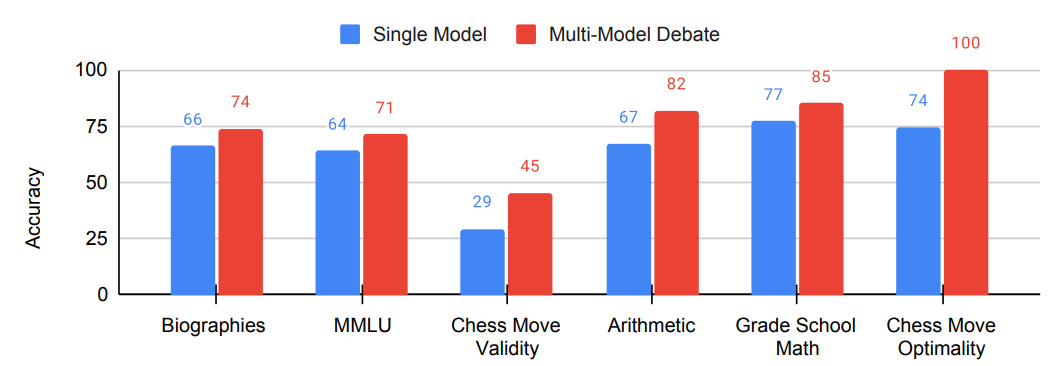
\includegraphics[width=1\linewidth]{img/section_background/multi-agent-debate-result.png}
    \caption{{Multiagent Debate Improves Reasoning and Factual Accuracy}}
    \label{fig:multiagent}
\end{figure}

Although this result is surprising, the performance of the multi-agent debate system plateaus as the number of agents or rounds increases, eventually converging to a certain level (see Figure \ref{fig:performance_with_increased}). Based on these observations, we hypothesize that incorporating dynamic, hierarchical communication topologies could further enhance the system. To implement the debate system and its communication topology, we leveraged the Autogen framework\cite{microsoft_autogen}, which provides the flexibility to define both the topology and the agents’ behavior.
\begin{figure}
    \centering
    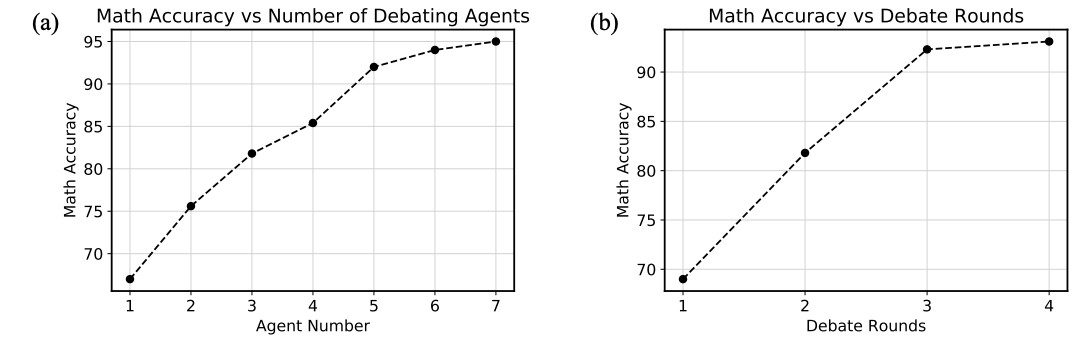
\includegraphics[width=0.85\linewidth]{img/section_background/performance_with_increased.png}
    \caption{(a) Performance with Increased Agents. (b) Performance with Increased Rounds}
    \label{fig:performance_with_increased}
\end{figure}